\chapter{Introduction}\label{ch:introduction}
This project does not stand alone. It has been built upon decades of research and has been strongly influenced by several external factors. In this chapter, we will present the social framework in which it has been developed and then particularize why it might be relevant for robotics and computer vision communities. After contextualizing our work, we will set the goals pursued during its development and describe the methodology followed to achieve them. For ease of reading, we will conclude this chapter with a brief overview of this report structure.

\section{Context and motivation}\label{ch:context_and_motivation}
% 4th industrial revolution
In recent years, we have assisted to an unprecedented process of digitization of data from the most diverse sources, which has been coupled with a very significant increment in computational capacity. We are immersed in what has
come to be called the \emph{Fourth Industrial Revolution}~\cite{schwab2017fourth}. This revolution has reached, to some extent, all areas of society, \eg health services, sports, education, finance, marketing, security or transport. In that sense, cross-sectional fields such as robotics have been immensely affected by these changes.

% robotics
If we think about the nature of most robotics applications, they usually have strong requirements in terms of how fast the robot must take action given streams of data that must be integrated and interpreted. On top of that, a lot of these applications demand the robot to be portable and lightweight (\eg drones or vacuuming robots). Taking these considerations into account, it is clear how heavily robotics rely on the development of very agile algorithms that can be embedded in computers with limited resources, even though these resources are not as limited as they once were.

% human robot interaction
One of the subfields in robotics that has received most attention lately is \gls{hri}. As a core component of robotics applications in areas such as assistive robotics, search and rescue or home automation, \gls{hri} is attracting interest from both academy and industry~\cite{Goodrich2007}. It is in itself a very interdisciplinary field of study, where researchers with expertise in multiple areas of engineering, natural language or psychology have come together to better understand the processes involved in the interaction between humans and robots in order to design increasingly intelligent systems. 

% human robot interaction levels
Communication between humans and robots may appear in many forms. In Figure~\ref{fig:hri}, examples of different forms of interaction are shown. In one side of the spectrum, it can mimic communication between humans, as it can be seen in the case of humanoid robots built for companionship. In the opposite side, it can be a very direct one-way communication. Such is the case of robot teleoperation, where the human acts as supervisor or operator. In between these, we can find applications in which the human teaches a robot to perform a task or vice versa; or those in which humans and robots work together as peers in industrial environments (\emph{cobots}). In any of these cases, robots must present some kind of human-aware behaviors. In order to gain this kind of awareness, robotic systems rely on the streams of data provided by their sensors, being the most common audio and video signals, which are used for enabling verbal and non-verbal communication, respectively. 

\begin{figure}[h]\centering
    \begin{subfigure}{0.34\textwidth}\centering
        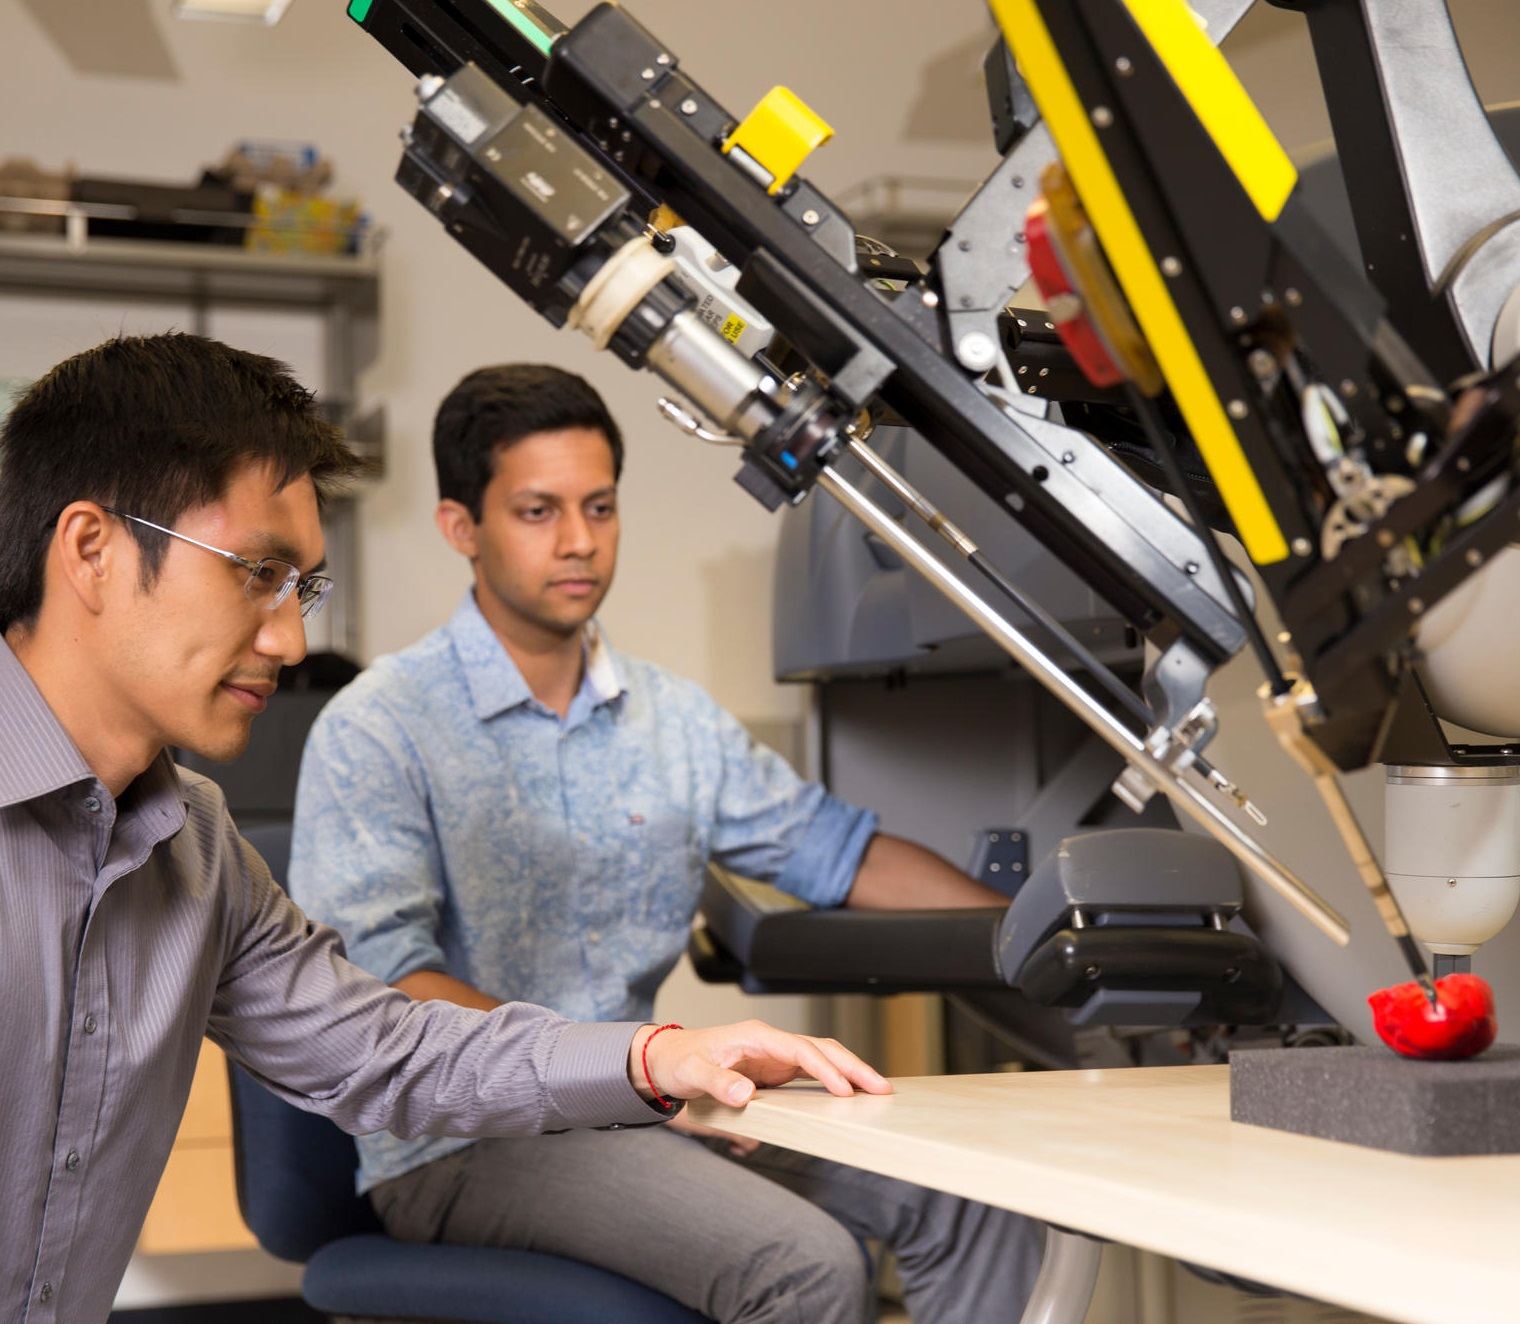
\includegraphics[height=4.5cm]{figures/teleoperated.jpg} 
        \caption{ARCLab surgical robot~\cite{arclab_2019}.}
        \label{subfig:teleoperated}
    \end{subfigure}
    \begin{subfigure}{0.2\textwidth}\centering
        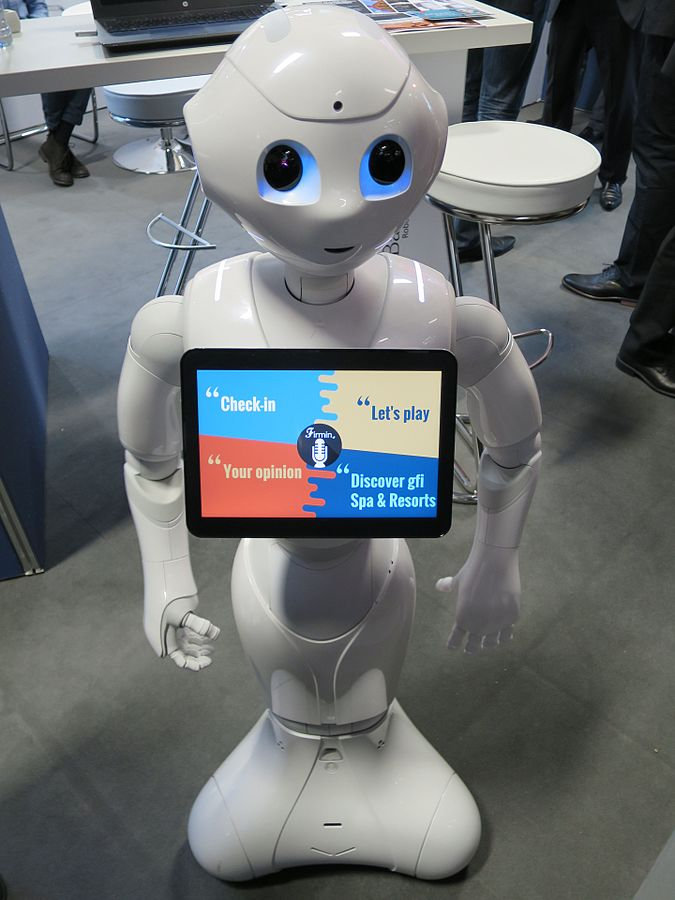
\includegraphics[height=4.5cm]{figures/companion.JPG}
        \caption{Pepper~\cite{travelarz_2017}.}
        \label{subfig:companion}
    \end{subfigure}
    \begin{subfigure}{0.41\textwidth}\centering
        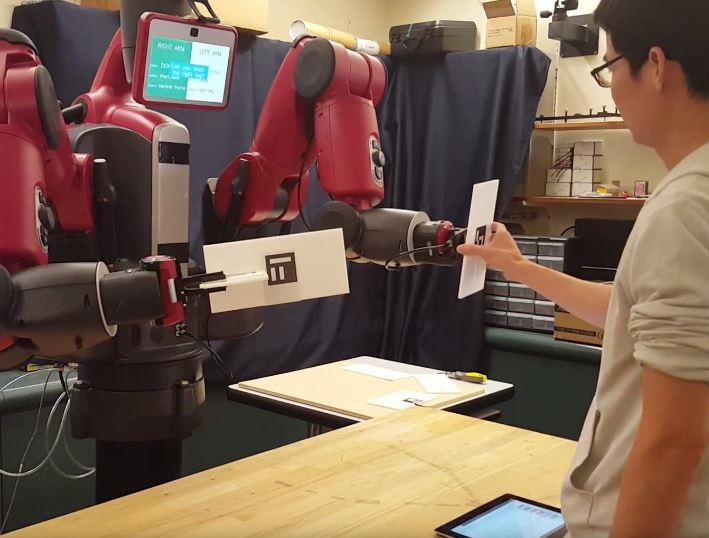
\includegraphics[height=4.5cm]{figures/collaboration.JPG}
        \caption{Baxter~\cite{roncone2017transparent}.}
        \label{subfig:companion}
    \end{subfigure}
    \caption{Human-robot interaction can take many forms. From left to right, we present examples of (a) teleoperation, (b) companionship and (c) collaboration.}
    \label{fig:hri}
\end{figure}

% computer vision + human pose estimation
From video signals, useful information can be extracted by analyzing the subject and its environment. These kinds of analysis are dependent on subfields of computer vision, such as human pose estimation, human detection and gesture recognition~\cite{leo2018deep}. In particular, human pose estimation is a very helpful capability for human-aware robots, since it can serve as an input for solving higher level tasks. For instance, a robot could watch a human peer to avoid collisions or could detect if the human has fainted and alert the emergency services. Broadly speaking, a precise identification of human pose provides a better understanding of the scene, which is a major requirement for any human-robot interface.

% mocap and classic approaches
\gls{mocap} systems are a well known solution for human pose estimation~\cite{vicon_2020}. They provide very precise 3D coordinates and are used in both commercial and academic environments, as shown in Figure~\ref{fig:mocap}. As a major drawback, they usually rely on markers placed on the humans to be tracked and multiple cameras or sensors around the scenario. Typically, these cameras are close to the ceiling in order to have a high point of view and cover the area to monitor~\cite{leone2011detecting}. The larger the area to monitor, the greater the number of needed cameras. \gls{mocap} systems are therefore very cumbersome and involve high installation costs, which prevents their usage as part of robotics applications, as the already mentioned assistive or industrial robots. In general, any robot that needs to be portable or distributed massively in commercial applications, requires more lightweight solutions in terms of both hardware and software. 

\begin{figure}[h]\centering
    \begin{subfigure}{0.49\textwidth}\centering
        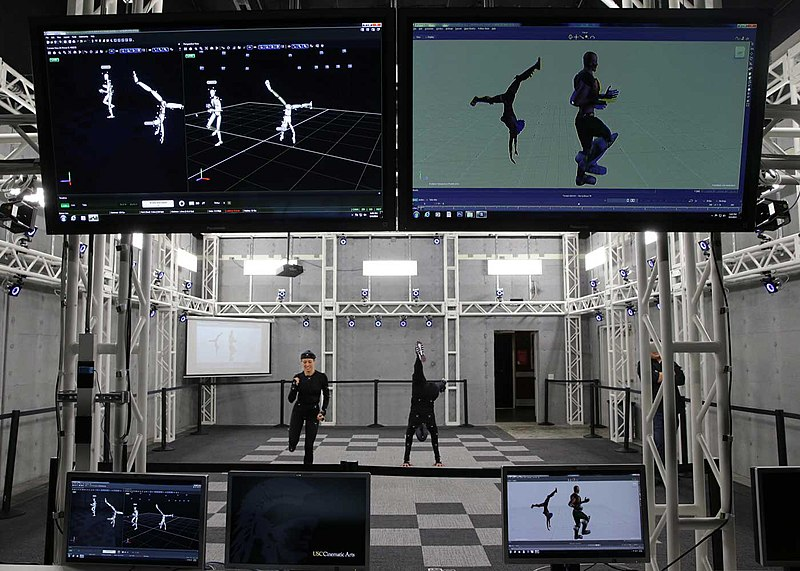
\includegraphics[height=5.5cm]{figures/optitrack.jpg} 
        \caption{\emph{OptiTrack} commercial MoCap system~\cite{optitrack_2019}.}
        \label{subfig:optitrack}
    \end{subfigure}
    \begin{subfigure}{0.49\textwidth}\centering
        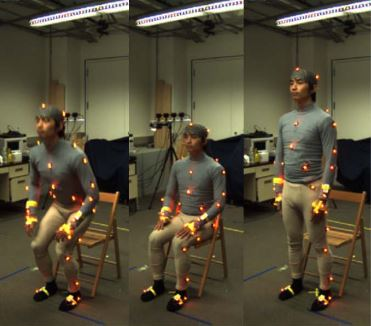
\includegraphics[height=5.5cm]{figures/bmhad_example.JPG}
        \caption{MoCap system in \emph{UC Berkeley}~\cite{ofli2013berkeley}.}
        \label{subfig:berkeley}
    \end{subfigure}
    \caption{MoCap systems are reliable solutions for both (a) commercial and (b) academic applications.}
    \label{fig:mocap}
\end{figure}

% machine learning, deep learning
Coming back to the so-called \emph{Fourth Industrial Revolution}, one of the fields of study that has benefited the most from the increase in data availability and computational capacity is \gls{ml}, and more specifically \gls{dl}. As stated by Andrew Ng~\cite{ng2016nuts}, scale drives \gls{ml} progress, in the sense that as computational capabilities scale, so does the amount of data that can be used to improve the performance of the algorithms developed. In other words, as the amount of data available increases, so does the computational power needed to maximize the performance of \gls{ml} algorithms. That is why, even if the core principles of \gls{dl} solutions, such as \glspl{nn}, were developed a long time ago, the field did not start to get its well deserved attention until the requirements of data and computational capacity where met in the last decade. These advances, coupled with major breakthroughs in training algorithms, have positioned \gls{dl} as the best approach for solving tasks which are highly dependent on robustness when dealing with real-world data. Such is the case of fraud detection, speech and face recognition or autonomous driving, just to mention a few ones~\cite{liu2017survey}.

% dl in computer vision and human pose estimation
Computer vision is one of the areas for which \gls{dl}-based solutions have entailed a greater improvement in terms of performance. Particularly, \glspl{cnn} have unseated classic computer vision algorithms as the best solution for solving some of the hardest problems in the field, including human pose estimation. Unlike classic \glspl{nn}, \glspl{cnn} take advantage of the spatial relationship between variables that are close to each other, allowing for translation invariance. In that way, they are specially suitable for processing \emph{grid-like} data such as pixels in an image or time-steps in an audio signal. Besides their effectiveness, they can be really fast during inference, even though training can take a long time. Given that a \gls{gpu} is available for acceleration, \gls{dl} algorithms can be embedded into a robot and work in real-time. A very illustrative case of success in the usage of \glspl{cnn} for performing human pose estimation is \emph{OpenPose}~\cite{cao2018openpose}, an open-source real-time system for multi-person 2D pose estimation, which is often used as a base component for building higher level applications. An example of \emph{OpenPose} impressive performance \textit{in the wild} is shown in Figure~\ref{fig:openpose}.

\begin{figure}[h]
    \centering
    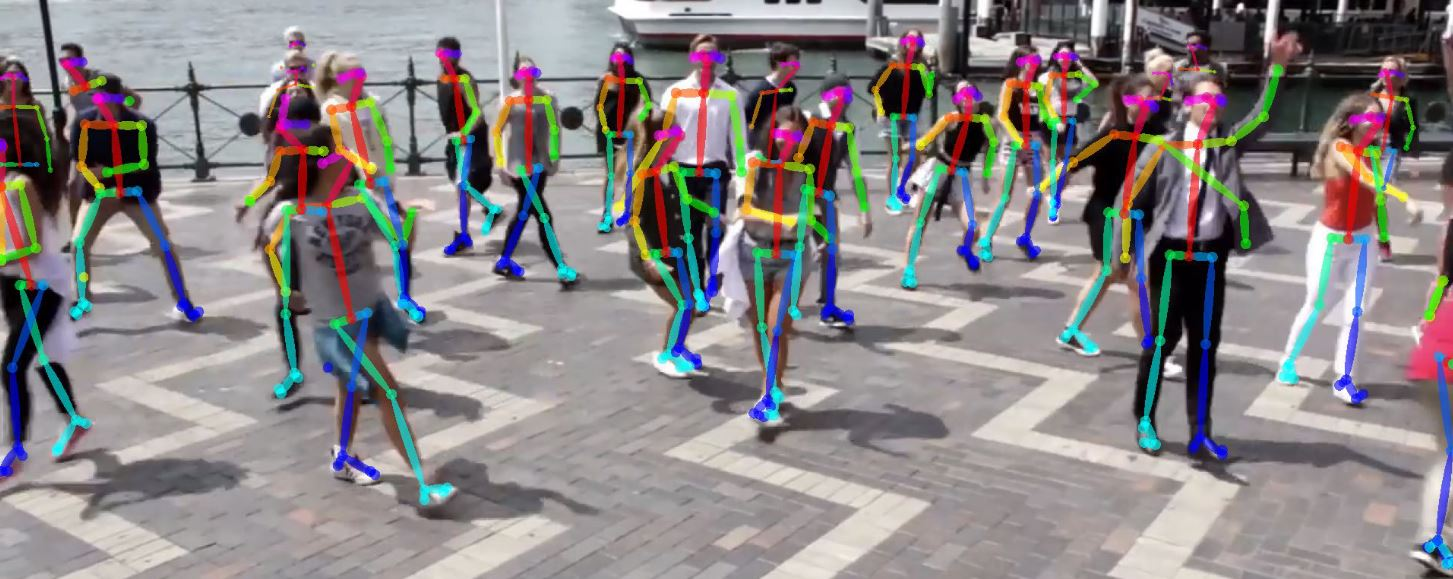
\includegraphics[width=\textwidth]{figures/openpose.JPG}
    \caption{Multi-person 2D poses estimated by \emph{OpenPose} system in real-time~\cite{cao2018openpose}.}
    \label{fig:openpose}
\end{figure}

% challenges, lack of 3D datasets in the wild
While the irruption of \gls{dl} has had an undeniably beneficial impact in the development of the field of human pose estimation, the needed amount of real-world data for designing models achieving a good performance is still an issue, as capture and annotation processes are costly and very time consuming. This is specially true for 3D images, where motion capture systems are usually needed for collecting reliable annotations~\cite{ionescu2013human3, sigal2010humaneva}. As a consequence, there is a strong gap in the number of publicly available large-scale datasets in favor of the two-dimensional ones. While 2D estimations might be enough for solving some particular tasks like action recognition~\cite{liu2018recognizing}, 3D estimations are needed in order to achieve a complete visual understanding of the scene~\cite{Sarafianos2016}. Fortunately, the emergence of robust RGBD sensors at affordable prices, such as \emph{Microsoft Kinect}~\cite{zhang2012microsoft} or \emph{Asus Xtion}~\cite{xtion}, allows the integration of real 3D data into human pose estimation pipelines. Along with these sensors, companies usually provide easy to use \glspl{sdk} and drivers, what favors their inclusion as part of the equipment of robots in the industry.

\section{Goals}\label{sec:goals}
In this work, we will design and develop an \emph{end-to-end} pipeline for augmenting 2D human pose estimations into 3D estimations. This perceptive algorithm is intended to be run on-board in robotics systems, so it must fulfill the following requirements:
\begin{itemize}
    \item It must work in real-time in an \emph{off-the-shelf} computer.
    \item It must work with a single regular RGBD camera, which is a commonly used sensor in robotics.
    \item It must work independently of the camera point of view, as the robot might move around the scene.
\end{itemize}

We will validate its usability and perform a wide and detailed comparison with some of the most relevant human pose estimation algorithms in the \gls{sota}. These comparisons will be carried out using \gls{bmhad} as benchmark, which is a publicly available and well-known international dataset~\cite{ofli2013berkeley}. Therefore, the main goals of this project can be summarized as follows:
\begin{enumerate}
\item Quantitative evaluation and comparison of multiple \gls{sota} methods for 2D human pose estimation, which will be included as the base of our 3D estimation pipeline.
\item Design and development of a straight-forward method for augmenting 2D estimations into 3D estimations in real-time using RGBD sensors.
\item Quantitative evaluation and comparison of our 3D human pose estimation method and a \gls{sota} algorithm.
\item Qualitative evaluation of the performance of our proposed pipeline with a real-time demo running in an \emph{off-the-shelf} laptop with a single regular RGBD sensor.
\end{enumerate}

\section{Methodology}\label{ch:methodology}
The development of this project has been weekly followed by its supervisors. During each meeting, results from the previous week were discussed and goals for the next one were established. In that way, we have been able to rapidly adjust to unexpected issues along the way. Furthermore, the frequent open discussions during these meetings have enabled a deeper understanding of the studied problem.

Besides the weekly meetings, the following external tools have been used to keep track of the progress of this project:
\begin{itemize}
    \item \textbf{Blog.} A blog hosted in the \emph{Robotics Lab URJC} platform~\footnote{\url{https://roboticslaburjc.github.io/2017-tfm-david-pascual/}} has been maintained as a logbook of each week advances.
    \item \textbf{\emph{GitHub}.} We have used \emph{Git}~\footnote{\url{https://git-scm.com/}} for our software version control. Enforcing \emph{open-source} practices, our main repository is hosted in \emph{GitHub} and is publicly available~\footnote{\url{https://github.com/RoboticsLabURJC/2017-tfm-david-pascual}}. It contains not only the code developed to meet the goals defined in the previous section, but also this report and the aforementioned blog.
\end{itemize}

Regarding software development, we have loosely followed an iterative model~\cite{larman2003iterative}. Instead of establishing a full list of specifications to reach a final version of the software, a small list of basic requirements has been set for each new iteration. After each of these, a functional version of the project has been presented and new requirements have been established. This iterative process forces the developer to divide the pending work in smaller, more manageable chunks. It also increases flexibility, as it allows to reduce or extend the scope of each iteration as needed. This kind of methodology may become messy if the software is developed by larger teams, but is very well suited for small ones.

\section{Project structure}\label{ch:project_structure}
For ease of reading, the structure of the report and a brief description of the contents of each chapter is presented here.

\begin{description}
\item[Chapter~\ref{ch:introduction}. Introduction.] In this chapter, we describe the context in which this project has been developed. Furthermore, our main goals are defined, along with the methodology followed to achieve them.
\item[Chapter~\ref{ch:related_work}. Related work.] Relevant human pose estimation algorithms, from classic approaches to the most recent ones, are described and categorized depending on the data used as input and the nature of their estimations.
\item[Chapter~\ref{ch:proposed_method}. Proposed method.] Our proposed algorithm takes as input 2D pose estimations and augments them to 3D using RGBD sensors. In this chapter, we give an overview of the tested 2D pose estimation methods and describe in detail the steps of our augmentation pipeline.
\item[Chapter~\ref{ch:experiments}. Experiments.] A wide quantitative comparison of 2D and 3D estimation methods is performed, both in terms of accuracy and computational burden. Besides that, we present a demo showcasing the proposed pipeline.
\item[Chapter~\ref{ch:conclusions}. Conclusions and future lines.] Finally, we look back into the work we have performed and discuss to which extent the proposed goals have been accomplished, highlighting the pros and cons of our system and giving an outline of potential future work.
\end{description}